\chapter{\umld}
\label{chap:UMLDesigner}

\section{Description}

\umld is an open-source tool to edit and visualize UML2 models created by the French company:
\textit{Obeo}. The project is licensed under the EPL\footnote{Eclipse public license}

\begin{figure}[h] \centering
  
\includegraphics[width=0.3\textwidth]{logo}
  \caption{UML Designer logo}
  \label{fig:logo}
\end{figure}

\section{Utilization}

\umld is a graphical modeling tool for UML2 as defined by OMG\footnote{Object Management Group\cite{omg}}. As
you can see on the figure \ref{fig:umldesigner}, it permit to create diagram on which ones it is
possible to add some elements. The type of the elements proposed depend on the types of the diagram
chosen. For example, if you choose a \textit{User case diagram} it is possible to add 'user'
component that is impossible in \textit{Class diagram}.

So with graphical action it is possible to create many UML diagram which have transverse elements.

To finish, it is possible to create the code of the application that you have develop from the
model.


\begin{figure}[h] \centering
  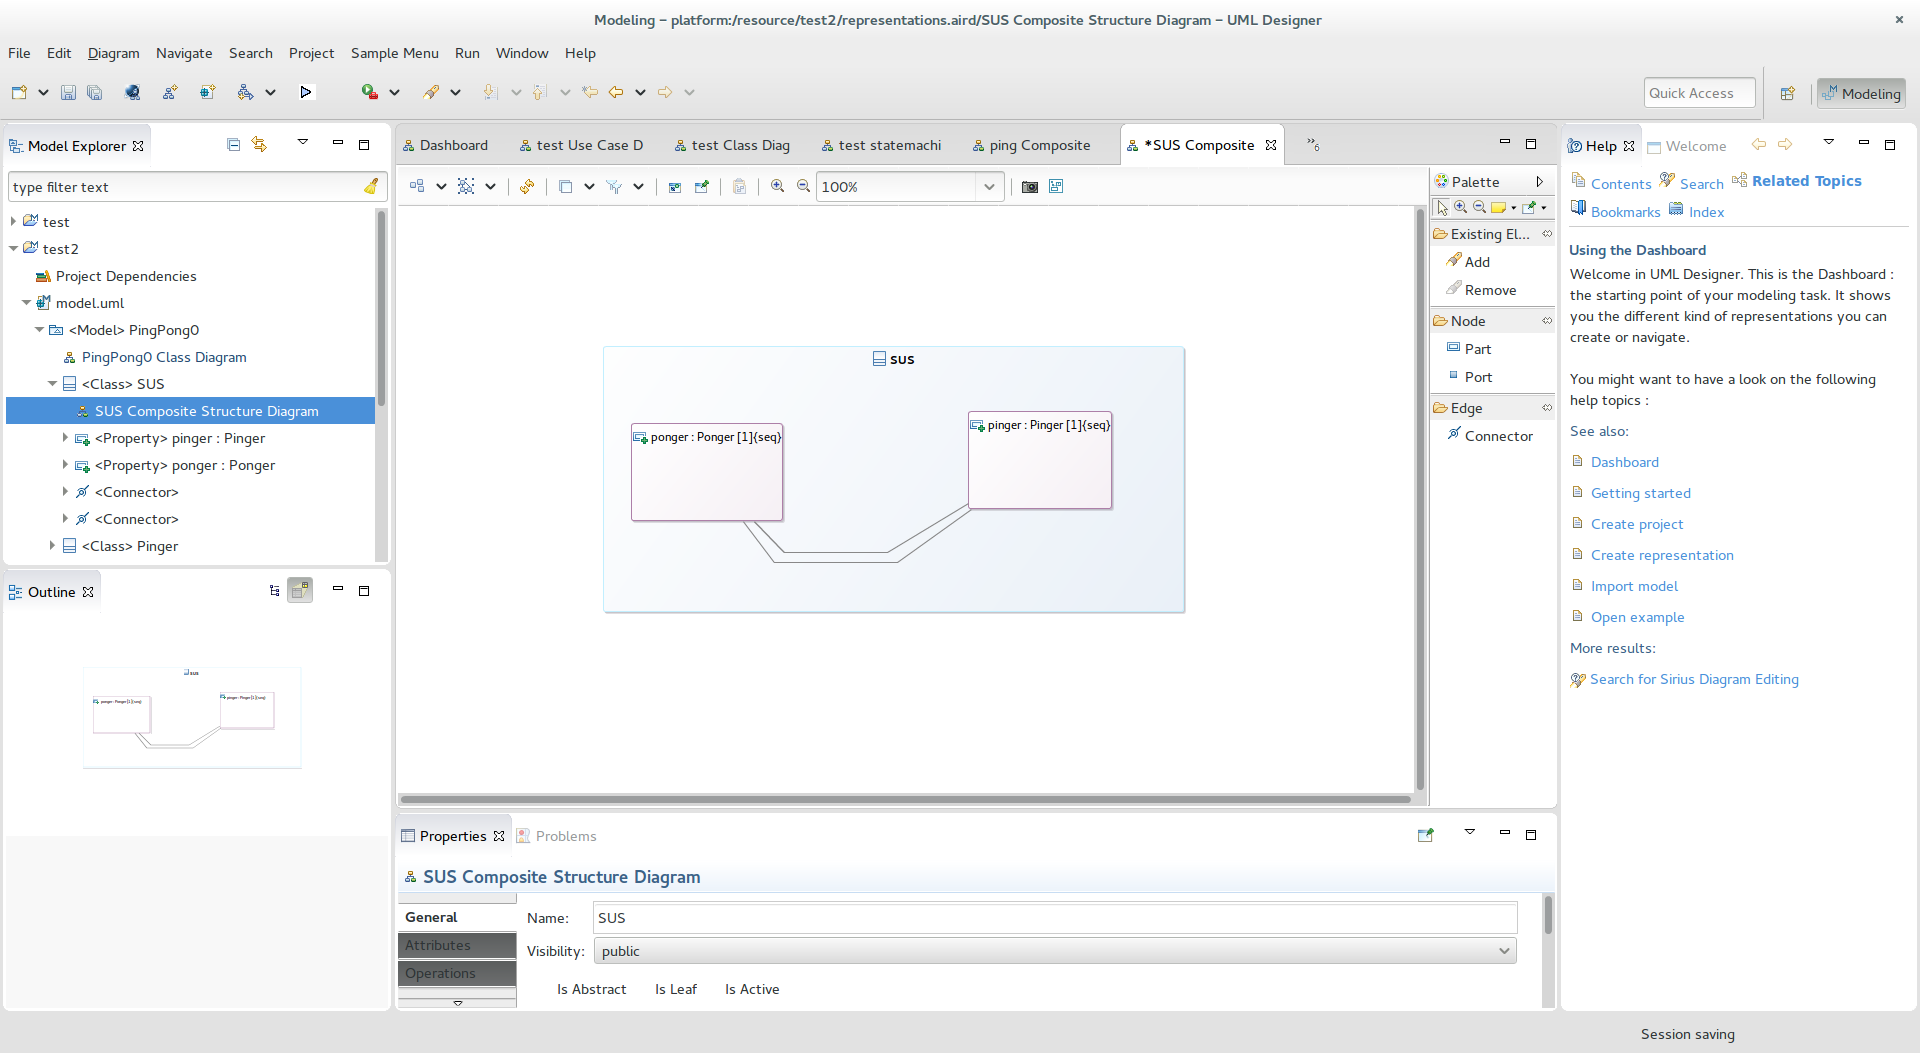
\includegraphics[width=0.8\textwidth]{umldesigner}
  \caption{Screen shot of \umld}
  \label{fig:umldesigner}
\end{figure}



\section{List of diagram supported}

\begin{itemize}
\item Packages diagram
\item Use case diagram
\item Activity diagram
\item Class diagram
\item Component diagram
\item Composite Structure diagram
\item Sequence diagram
\item State Machine diagram
\item Documentation table
\item Use Case cross table
\item Package containment diagram
\item Profile diagram
\end{itemize}



\section{Released}
\begin{center}

  \begin{tabular}{|c|c|}
    \hline
    \textbf{Version} & \textbf{Release Date} \\
    \hline
    1.0.0 &2012\\
    \hline
    2.0.0 &17 January 2013\\
    \hline
    2.1.0 &1 February 2013\\
    \hline
    2.2.0 &12 April 2013\\
    \hline
    2.3.0 &13 June 2013\\
    \hline
    2.4.0 &13 September 2013\\
    \hline
    3.0.0 &17 January 2014\\
    \hline
    4.0.0 &8 July 2014\\
    \hline
    4.0.1 &5 August 2014\\
    \hline
    5.0.0 &29 May 2015\\
    \hline
    \cellcolor{green}6.0.0 &19 October 2015\\
    \hline
  \end{tabular}

  \begin{tabular}{c}
    Legend:\\
    \cellcolor{green}Latest stable release\\
  \end{tabular}

\end{center}

\section{Base on}

\umld is based on a Eclipse and Sirius. It is a UML2 Eclipse plugin.

\subsection{Sirius}
Sirius is an open-source software project of the Eclipse Foundation. Sirius allows to create graphical modeling workbench. It include EMF\footnote{Eclipse Modeling Framework} and GMF\footnote{Graphical Modeling Framework}. On the figure \ref{fig:sirius}, it is possible to see the architecture of Sirius.


\begin{figure}[h]
  \centering
  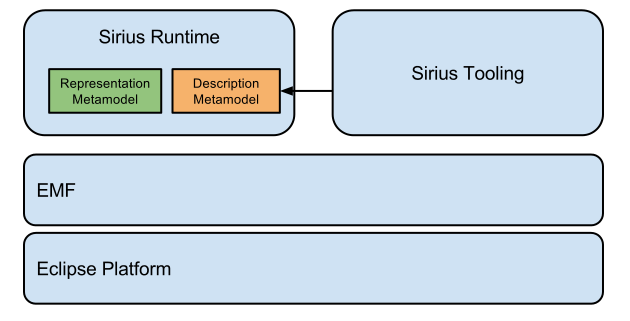
\includegraphics[width=\textwidth]{sirius_archi}
  \caption{Sirius architecture\cite{sirius}}
  \label{fig:sirius}
\end{figure}

\subsection{Eclipse}

\umld is base on Eclipse.
The interface is the same as Eclipse. You can notice on figure
\ref{fig:umldesigner} that the menu are the same in the both software.



\begin{figure}[h] \centering
  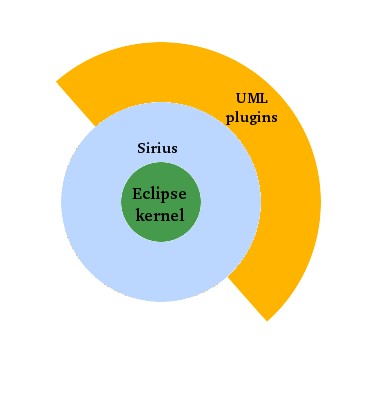
\includegraphics[width=0.5\textwidth]{archi}
  \caption{The \umld kernel}
  \label{fig:kernel}
\end{figure}






%%% Local Variables:
%%% mode: latex
%%% TeX-master: "../rapport_de_base"
%%% End:
